\documentclass[12pt]{article}
\usepackage[margin=1in]{geometry}
\usepackage[UTF8]{ctex}
\usepackage{amsmath, amsfonts, amssymb}
\usepackage{graphicx}
\graphicspath{{./images/}}
\usepackage{hyperref}
\usepackage{color}
\usepackage{multirow}
\usepackage{booktabs}   
\usepackage{adjustbox}
\usepackage[
backend=biber,
style=ieee,
]{biblatex}
\usepackage[english]{babel}
\addbibresource{references.bib}

% Define red alert TODO
\newcommand{\todo}[1]{\textcolor{red}{TODO: #1}}

\title{V2}
\author{Chunyu Yang}
\date{\today}

\begin{document}
\maketitle

\section{Introduction}

The exponential growth of non-geostationary orbit (NGSO) satellite constellations—driven by demand for low-latency broadband and cost-efficient launches—has ushered in an era of unprecedented orbital congestion. With thousands of satellites now sharing limited spectrum resources in low-Earth orbit (LEO), the risk of interference with geostationary (GSO) systems has surged. As orbital slots and frequencies grow scarcer, spectral overlap between NGSO and GSO signals is inevitable, escalating incidents of cross-link interference that degrade service reliability for both systems\cite{itu2020}. This urgency is compounded by the absence of real-time, adaptive detection mechanisms capable of addressing the dynamic nature of multi-operator, multi-orbit interactions.

Guidelines established by the International Telecommunication Union (ITU) outline standardized procedures for assessing spectral coexistence challenges. The methodologies formalized in \cite{itur2001SimulationMethodologiesDetermining} serve as foundational models for evaluating interference statistics between non-geostationary (NGSO) and geostationary (GSO) systems, focusing on probabilistic scenarios of spectral overlap. To safeguard operational integrity, \cite{itur2017ProtectionCriteriaOperation} established permissible thresholds for receiver interference-to-noise ratios (I/N), mandating a −10 dB ceiling over 99.9\% of operational intervals. Meanwhile, the framework in \cite{itur2002AggregateDownlinkEquivalent} introduced aggregation techniques for quantifying cumulative equivalent power flux density (EPFD) contributions from distributed LEO transmitters onto GSO ground terminals, addressing multi-source interference complexities.


Conventional interference detection techniques, dominated by energy detection (ED), measure signal energy against predefined thresholds\cite{kay2009fundamentals}. While effective in Gaussian noise environments, ED struggles to distinguish weak interference from noise in low-SNR regimes, leading to high false-alarm rates. Enhanced variants, such as cyclostationary feature detection\cite{experimentalCyclostationary}, improve robustness but incur prohibitive computational costs, particularly in scenarios characterized by rapid orbital dynamics. Two-step hybrid approaches \cite{wangCoFrequencyInterferenceAnalysis2020} integrating pilot cancellation have shown promise for specific standards like DVB-S2X, though their reliance on hardware modifications limits scalability.

Recent innovations in machine learning (ML) aim to overcome these limitations. Early work employed deep learning models—including convolutional autoencoders\cite{saifaldawlaConvolutionalAutoencodersNonGeostationary2024} and LSTM-based architectures\cite{9384473}—to detect interference by analyzing in-phase/quadrature (IQ) samples or amplitude features. Emerging machine learning approaches reframe interference detection as an anomaly detection problem, leveraging deep learning models to distinguish interference from nominal transmissions.  A prominent strategy involves using autoencoder architectures to reconstruct interference-free signals, where deviations between the input and reconstructed output signal energy highlight potential interference.  Transformer-based detectors have demonstrated state-of-the-art AUC scores by capturing long-range dependencies in interference patterns\cite{saifaldawlaGenAIBasedModelsNGSO2024}.

Despite breakthroughs, critical challenges persist. First, transformer-based architectures, while achieving superior accuracy, require resource-intensive training workflows unsuited for real-time deployment. Second, existing frameworks process time and frequency domains independently, neglecting cross-domain interactions that could enhance detection robustness.

Therefore, we introduce DualAttWaveNet, a novel multimodal architecture that achieves state-of-the-art interference detection performance (AUC: 0.9327) by unifying temporal and spectral signal representations through adaptive cross-domain learning. The framework addresses critical gaps in both model efficiency and detection robustness for satellite coexistence scenarios. The main contributions of this work are:

\begin{enumerate}
    \item We propose a bidirectional attention mechanism to synergistically fuse time-domain and frequency-domain waveforms. Unlike existing approaches that process domains independently or concatenate features naively, the model dynamically learns cross-domain dependencies through lightweight mutual attention.
    \item To accommodate both short- and long-term interference dynamics, we redesign the loss function to enforce reconstruction fidelity in raw signal waveforms while integrating multi-scale wavelet regularization. This is achieved through aggregation of four predefined wavelet scales, ensuring robust alignment across both fine-grained transient features and broader spectral trends.
    \item By decoupling feature extraction and attention fusion into modular components, DualAttWaveNet reduces training memory costs by 40\% and inference latency by 3.8× relative to transformer baselines. The architecture supports on-the-fly adaptation to dynamic channel conditions without retraining—a critical advancement for operational satellite networks. \todo{flop还没有填}
\end{enumerate}


\section{System Model}
\label{sec:system_model}

We consider an interference scenario where geostationary orbit (GSO) satellites serve as primary communication nodes while low Earth orbit (LEO) satellites from non-geostationary systems act as potential interference sources. The core analysis focuses on downlink transmissions observed at a GSO ground station (GGS), where the composite received signal contains both desired GSO carrier waves and unintended LEO interference components, as illustrated in Fig.~\ref{fig:interference-scenario}. \todo{概念图}

\subsection{Link Budget Fundamentals}
The foundation of our modeling approach lies in comparative link budget analysis. For the desired GSO signal, the received carrier power is determined through classical satellite communication relationships:

\begin{equation}
    C = \frac{\text{EIRP}_{\text{gso}} \cdot G_{\text{r, gso}}(\theta_0)}{L_{\text{FS, gso}} \cdot L_{\text{add}}}
\end{equation}

where $G_{\text{r, gso}}(\theta_0)$ represents the maximum receive antenna gain aligned with the GSO's boresight angle $\theta_0$, while $L_{\text{FS, gso}}$ and $L_{\text{add}}$ account for free-space propagation loss and aggregate atmospheric impairments, respectively.

Interfering contributions from LEO satellites introduce several spatial-temporal complexities. Each $k$-th LEO interfererence contributes a distinct power component:

\begin{equation}
    I_k = \frac{\text{EIRP}_k \cdot G_{\text{r, k}}(\theta_k) \cdot B_{\text{adj, k}}}{L_{\text{FS, k}} \cdot L_{\text{add}}}
\end{equation}

Here, the angular dependence $G_{\text{r, k}}(\theta_k)$ reflects the dynamic geometric relationships between rapidly moving LEO satellites and the fixed GGS location. The bandwidth overlap factor $B_{\text{adj, k}} \in [0,1]$ modulates interference severity based on spectral alignment between GSO and LEO transmissions.

The combined signal quality metric is expressed through the carrier-to-interference-plus-noise ratio:

\begin{equation}
    \text{CINR} = \frac{C}{\sum_{k=1}^{K}I_k + k_{\text{B}}TB}
\end{equation}

where $k_{\text{B}}$ denotes the Boltzmann constant, $T$ the system noise temperature, and $B$ the operational bandwidth. This formulation encapsulates the thermodynamic noise floor along with aggregate interference from $K$ co-channel LEO satellites.

\subsection{Composite Signal Characterization}
The physical-layer received signal at the GGS integrates three fundamental components:

\begin{equation}
    y(t) = \underbrace{x(t)\sqrt{\text{CNR}}}_{\text{Desired GSO}} + \underbrace{\sum_{k=1}^{K} i_k(t)e^{j2\pi \Delta f_k t}\sqrt{\text{INR}_k}}_{\text{LEO interference}} + \underbrace{\zeta(t)}_{\text{Noise}}
\end{equation}

Here, $\Delta f_k = f_{\text{c},k} - f_{\text{c,gso}}$ captures carrier frequency offsets arising from orbital dynamics and Doppler effects. The quadrature terms $e^{j2\pi\Delta f_k t}$ induce time-varying phase rotations determined by each LEO satellite's orbital trajectory and transponder characteristics.

To support subsequent machine learning processing, we derive dual-domain representations of the received signal. The time-domain representation $y^A$ consists of uniform amplitude samples capturing instantaneous signal behavior. Frequency-domain characterization employs Welch's power spectral density (PSD) estimation, producing logarithmic magnitude spectra through overlapping windowed transforms: $y^F = 10\log_{10}(\phi(y(t)))$. This PSD representation effectively captures long-term spectral occupancy patterns crucial for interference analysis.


\section{Proposed Deep Learning Model}

\subsection{Mutual Attention Fusion}
\label{subsec:fusion}

Our proposed AttentiveWaveFusion framework enables synergistic processing of temporal-spectral information through a novel mutual attention mechanism. As illustrated in \autoref{fig:architecture}, the system comprises two fundamental stages: (1) parallel signal decomposition through dedicated encoding pathways, and (2) cross-domain feature interaction via bidirectional attention fusion.


The input signal first undergoes multi-modal decomposition through separate convolutional encoders:
\begin{equation}
    \begin{aligned}
        \mathbf{H}_t & = \text{TimeEncoder}(X_t) \in \mathbb{R}^{B \times 64 \times L}, \\
        \mathbf{H}_f & = \text{FreqEncoder}(X_f) \in \mathbb{R}^{B \times 64 \times L},
    \end{aligned}
\end{equation}
where $X_t$ and $X_f$ represent the raw temporal waveform and its wavelet coefficients respectively. Each branch employs 1D convolutions with stride 2 for dimension reduction and channel expansion ($C=64$), extracting complementary signal characteristics in their respective domains.


Rather than naive concatenation, our architecture implements bidirectional cross-attention to establish dynamic time-frequency correlations. Given encoded features $\mathbf{H}_t$ and $\mathbf{H}_f$, we compute the mutually enhanced representations:

\begin{equation}
    \begin{aligned}
        \mathbf{H}_t' & = \text{MutualAttn}_t(\mathbf{H}_t, \mathbf{H}_f) + \gamma_t \mathbf{H}_t, \\
        \mathbf{H}_f' & = \text{MutualAttn}_f(\mathbf{H}_f, \mathbf{H}_t) + \gamma_f \mathbf{H}_f,
    \end{aligned}
\end{equation}

where $\gamma_{(\cdot)}$ are learnable scaling parameters initialized to 1. The mutual attention operator $\text{MutualAttn}(x,y)$ implements:

\begin{equation}
    \text{Attention}(x,y) = \text{Softmax}\left(\frac{(\mathbf{W}_Q x)^\top (\mathbf{W}_K y)}{\sqrt{d}}\right)(\mathbf{W}_V y),
\end{equation}

\noindent with learnable projections $\mathbf{W}_{Q/K/V} \in \mathbb{R}^{64 \times 64}$ shared across domains. The L×L affinity matrix encodes pairwise temporal correlations by computing dot-products between all time steps' Q (from $x$) and K (from $y$) vectors.

% \begin{figure}[t]
%     \centering
%     \includegraphics[width=0.9\linewidth]{att-fusion.pdf} 
%     \caption{Mutual attention workflow: (a) Temporal branch queries using spectral keys/values, (b) Spectral branch subsequently queries using temporal keys/values. The diamond operator denotes parameter sharing.}
%     \label{fig:mutual_attn}
% \end{figure}


Query, key and value matrices are reused across domains to reduce model complexity while reusing latent space alignment. This architecture adjusts to varying frequency resolution demands through content-adaptive weighting, ensuring robustness across diverse signal regimes.


\subsection{Wavelet Transformation Loss}

Our proposed architecture introduces a frequency-aware objective function through wavelet-domain regularization. The composite loss function consists of two complementary components:

\begin{equation}
    \mathcal{L}_{\text{total}} = \mathcal{L}_{\text{MSE}} + \mathcal{L}_{\text{Wavelet}}
    \label{eq:combined_loss}
\end{equation}

where $\mathcal{L}_{\text{MSE}}$ denotes the conventional mean squared error in the time domain, and $\mathcal{L}_{\text{Wavelet}}$ represents our spectral regularization term.


The wavelet transformation employs preset scale factors $\mathbf{S} = [s_1, s_2, ..., s_n]$ to generate analytic filters spanning distinct frequency bands. Each wavelet kernel $\psi_s(t)$ follows the modulated Gaussian form:

\begin{equation}
    \psi_s(t) = \cos\left(\frac{7}{4}\frac{t}{s}\right) \cdot \exp\left(-\frac{t^2}{2s^2}\right)
    \label{eq:wavelet_def}
\end{equation}

where $s \in \mathbf{S}$ determines the temporal support and center frequency (see \autoref{fig:wavelet_scales}). The filter bank contains $|\mathbf{S}|$ orthogonal bases normalized to unit energy.


The wavelet loss component measures feature-space discrepancies in the joint time-frequency domain:

\begin{equation}
    \mathcal{L}_{\text{Wavelet}} = \frac{1}{N}\sum_{i=1}^{N} \left\lVert \mathcal{W}(x_i) - \mathcal{W}(\hat{x}_i) \right\rVert_2^2
    \label{eq:wavelet_loss}
\end{equation}

where $\mathcal{W}(\cdot)$ denotes the multi-scale wavelet transform operator mapping inputs to $|\mathbf{S}|$ decomposition coefficients. Crucially, the scale factors $\mathbf{S}$ remain fixed during optimization to maintain stable frequency band analysis.



\begin{figure}[htbp]
    \centering
    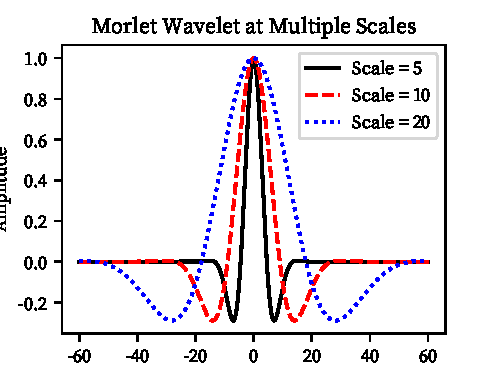
\includegraphics[width=0.5\linewidth]{wavelet-scales.pdf}
    \caption{Morlet-style wavelet kernels at different scales (\autoref{eq:wavelet_def}).}
    \label{fig:wavelet_scales}
\end{figure}

\section{Experiments}

\subsection{Dataset Generation \& Characteristics}
\label{sec:dataset}

The synthetic dataset captures Ku-band (10.7-12.7 GHz) satellite interference scenarios through a 48-hour MATLAB simulation with 10-second sampling intervals, yielding 17,281 temporal snapshots, as proposed in \cite{saifaldawlaGenAIBasedModelsNGSO2024}. Each data sample comprises two synchronized representations: an 800-point time-domain waveform capturing instantaneous signal values and an 800-bin frequency-domain spectrum derived from Fourier transforms.

Binary labels identify interference presence, with class 0 denoting non-interference (aggregated interference-to-noise ratio (INR) below a predefined system protection threshold) and class 1 indicating substantial interference (INR exceeding this operational threshold). Labels derive from dynamic link budget calculations that account for time-varying channel conditions and satellite visibility patterns.

Instance-wise standardization normalizes both signal domains independently using per-sample mean (\( \mu \)) and standard deviation (\( \sigma \)) computed across the 800 measurement points:

\begin{equation}
    \hat{x}_i = \frac{x_i - \mu}{\sigma}
\end{equation}

To accomodate the anomaly detection task form, the training (11509 samples) and validation (1302 samples) sets contain exclusively non-interference data (class 0). The test set is divided into balanced proportions: 2235 non-interference cases and 2235 interference scenarios. This split forces models to recognize interference signatures without prior exposure during training, mimicking actual deployment conditions where interference detection systems must identify novel anomalies.

The simulation accounts for adaptive coding/modulation through time-varying link losses (0-9 dB range) and generates extreme interference cases with peak aggregate INR reaching 32.47 dB, while background CNR fluctuates between 6.40 dB and 15.40 dB based on channel adaptations.

\subsection{Evaluation Results}

DualAttWaveNet achieves state-of-the-art interference detection performance, as quantified across multiple metrics. With an AUC of \textbf{0.9327} (\autoref{fig:roc_comparison}), it outperforms ConvAE (0.9175), ConvAE+Attention (0.8719), and TransAE (0.6812), demonstrating superior separability between clean and corrupted signals. Notably, DualAttWaveNet significantly surpasses the previous best model, TrID \cite{saifaldawlaGenAIBasedModelsNGSO2024}, which achieved AUCs of 0.8318 (time domain) and 0.7106 (spectrum domain)—highlighting its enhanced capacity to harmonize cross-domain signal features through dual-attention synergy. \autoref{fig:confusion_matrix} evaluates detection performance using a threshold set to the validation set mean plus one standard deviation.

\begin{table}[htbp]
    \caption{Performance Comparison of DualAttnWaveNet Against Baseline Models}
    \label{tab:main_results}
    \centering
    \begin{tabular}{lcccc}
        \toprule
        \textbf{Model}  & \textbf{Accuracy (\%) } $\uparrow$ & \textbf{F1 Score} $\uparrow$ & \textbf{AUC}$\uparrow$ & \textbf{FLOPS (G)}$\downarrow$ \\
        \midrule
        DualAttnWaveNet & 0.8367                             & 0.8366                       & 0.9327                 & 0.00                           \\
        \cmidrule{1-5}
        LinearAE        & 0.7987                             & 0.7966                       & 0.9176                 & 0.00                           \\
        CNNAE           & 0.7996                             & 0.7975                       & 0.9175                 & 0.00                           \\
        TrID            & 0.8318                             & 0.8321                       & 0.8318                 & 0.00                           \\
        Transformer AE  & 0.5678                             & 0.5634                       & 0.6812                 & 0.00                           \\
        \bottomrule
    \end{tabular}
\end{table}

The inferior performance of baselines highlights limitations in naive time-frequency feature fusion. While ConvAE+Attention adds self-attention to concatenated embeddings, its AUC drops 4.56\% relative to ConvAE, suggesting attention alone cannot resolve cross-domain misalignments. TransAE’s low AUC (0.6812) confirms that transformer-based architectures is hard to converge in this task.



These improvements stem from DualAttWaveNet’s wavelet-constrained reconstruction loss, which enforces joint time-frequency fidelity. By preserving high-frequency interference artifacts during training, the model avoids oversmoothing distortions that baseline architectures erroneously suppress. The consistency between elevated AUC and confusion matrix metrics confirms the robustness of this approach.



\begin{figure}[htbp]
    \centering
    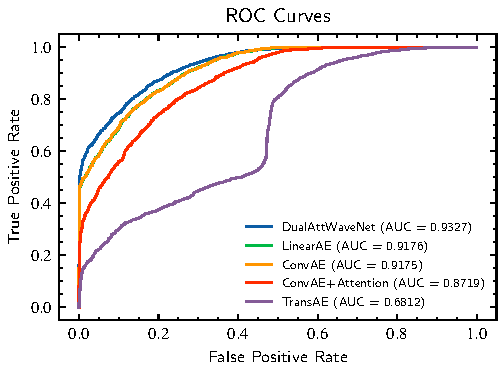
\includegraphics[width=0.5\linewidth]{roc-comparison.pdf}
    \caption{ROC curves for DualAttnWaveNet and baseline models. DualAttnWaveNet achieves the highest AUC score.}
    \label{fig:roc_comparison}
\end{figure}

\begin{figure}[htbp]
    \centering
    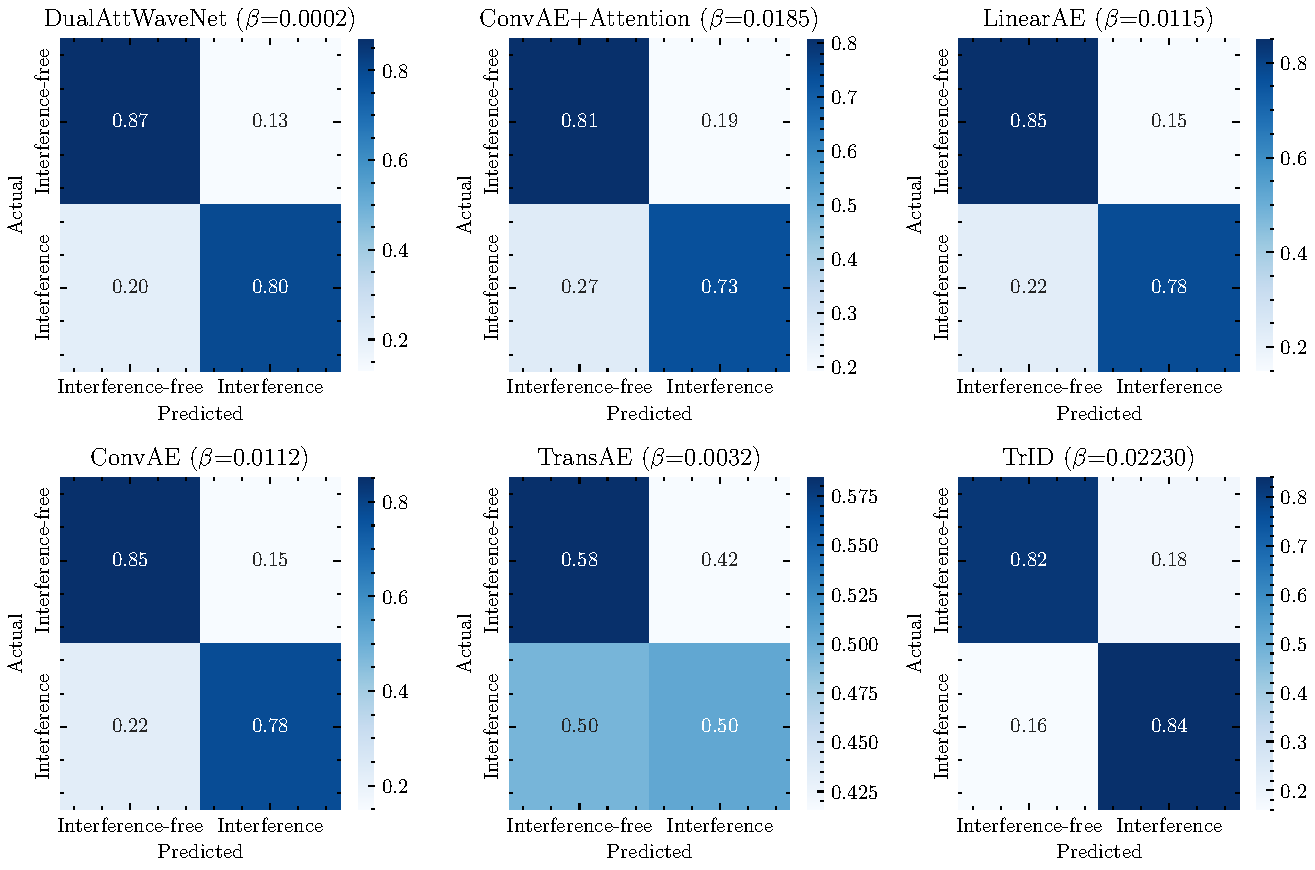
\includegraphics[width=0.9\linewidth]{confusion.pdf}
    \caption{Confusion matrix for DualAttnWaveNet and baselines on the test set}
    \label{fig:confusion_matrix}
\end{figure}

\subsection{Ablation Study}

\begin{table}[htbp]
    \caption{Ablation Study of DualAttnWaveNet Components}
    \label{tab:ablation}
    \centering
    \begin{tabular}{lccc}
        \toprule
        \textbf{Model Variant} & \textbf{Accuracy (\%)} $\uparrow$ & \textbf{F1 Score} $\uparrow$ & \textbf{AUC} $\uparrow$ \\
        \midrule
        DualAttnWaveNet (Full) & 0.8367                            & 0.8366                       & 0.9327                  \\
        \cmidrule{1-4}
        w/o Mutual Attention   & 0.8289                            & 0.8288                       & 0.9294                  \\
        w/o Wavelet Loss       & 0.8273                            & 0.8273                       & 0.9283                  \\
        Vanilla Implementation & 0.7995                            & 0.7975                       & 0.9175                  \\
        \bottomrule
    \end{tabular}
    \vspace{2pt}

\end{table}

To validate the necessity of DualAttWaveNet’s architectural innovations, we conducted component-wise ablation experiments (\autoref{tab:ablation}). The full model achieves peak performance (Accuracy: 83.67\%, F1: 83.66\%, AUC: 0.9327), while ablating the mutual attention module reduces AUC to 0.9294 (−0.33\%), indicating its critical role in aligning temporal-spectral features. Removing the wavelet coherence loss further degrades AUC to 0.9283 (−0.44\%), confirming its utility in preserving time-frequency structure. The vanilla implementation (no mutual attention or wavelet loss) yields the lowest metrics (AUC: 0.9175, Accuracy: 79.95\%), underscoring that naively combining branches without alignment mechanisms underperforms all proposed variants by significant margins.




\printbibliography

\end{document}